\begin{figure*}[hbtp]
  \centering
  \subfigure{
    \label{fig:im-key}
    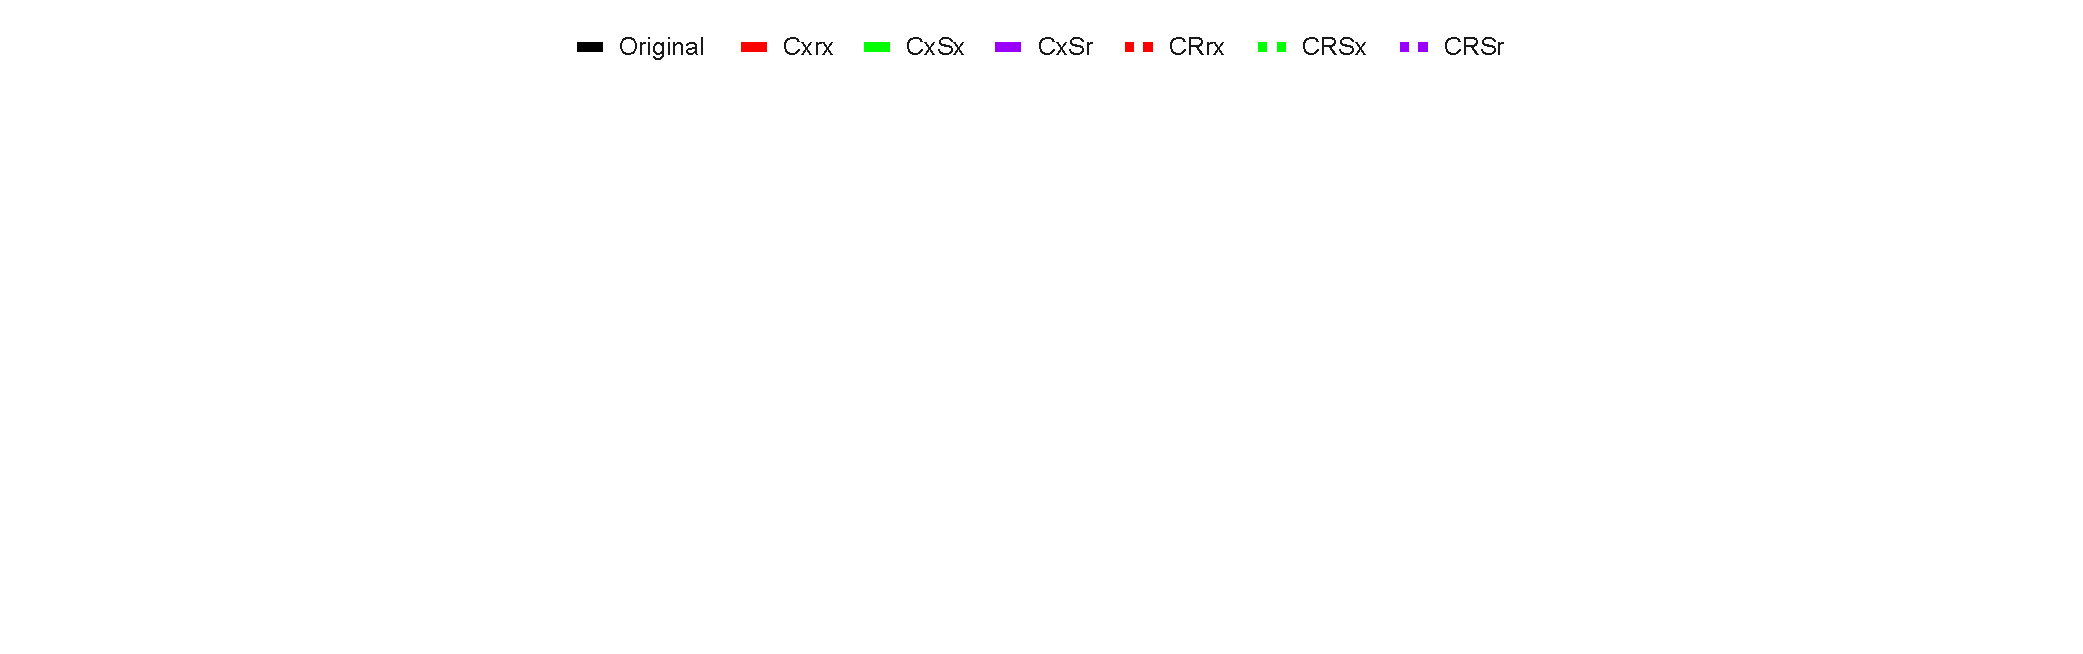
\includegraphics[width=0.98\linewidth]{out/im-key.pdf}
  } \\[-2ex]
  \subfigure{
    \label{fig:im-web-Stanford}
    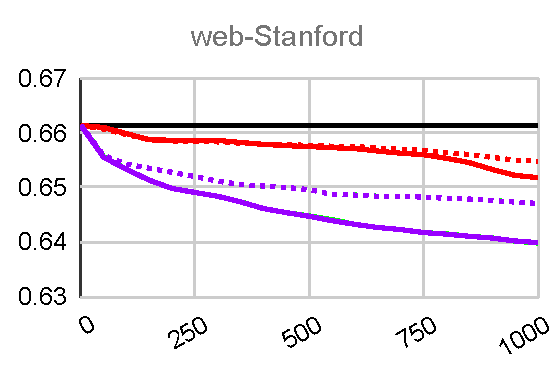
\includegraphics[width=0.23\linewidth]{out/im-web-Stanford.pdf}
  }
  \subfigure{
    \label{fig:im-web-BerkStan}
    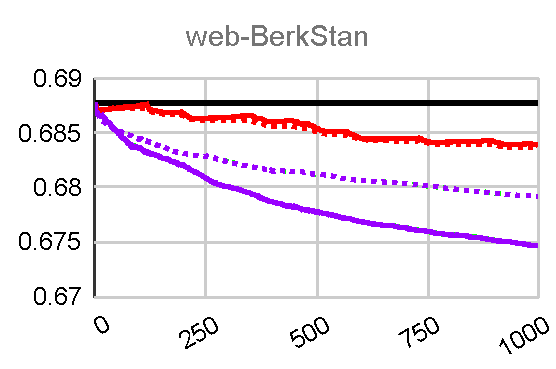
\includegraphics[width=0.23\linewidth]{out/im-web-BerkStan.pdf}
  }
  \subfigure{
    \label{fig:im-web-Google}
    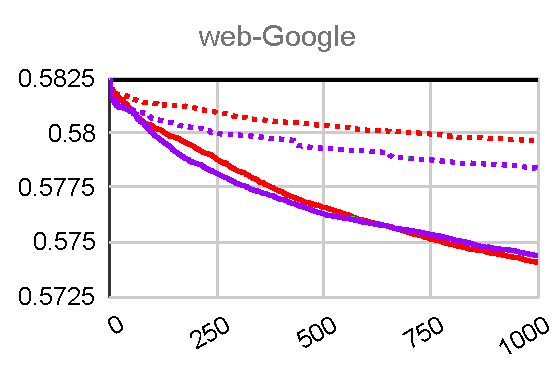
\includegraphics[width=0.23\linewidth]{out/im-web-Google.pdf}
  }
  \subfigure{
    \label{fig:im-web-NotreDame}
    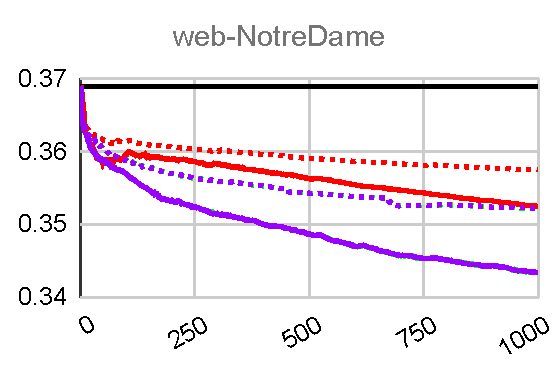
\includegraphics[width=0.23\linewidth]{out/im-web-NotreDame.pdf}
  }
  \subfigure{
    \label{fig:im-soc-Slashdot0811}
    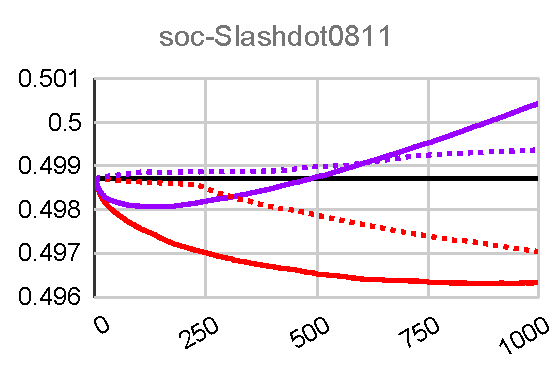
\includegraphics[width=0.23\linewidth]{out/im-soc-Slashdot0811.pdf}
  }
  \subfigure{
    \label{fig:im-soc-Slashdot0902}
    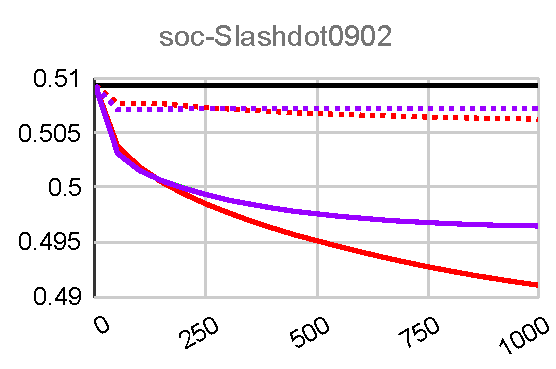
\includegraphics[width=0.23\linewidth]{out/im-soc-Slashdot0902.pdf}
  }
  \subfigure{
    \label{fig:im-soc-Epinions1}
    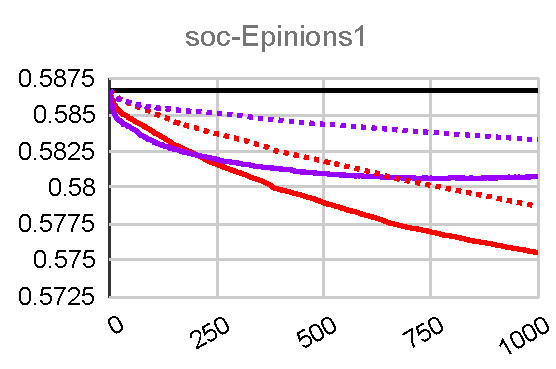
\includegraphics[width=0.23\linewidth]{out/im-soc-Epinions1.pdf}
  }
  \subfigure{
    \label{fig:im-soc-LiveJournal1}
    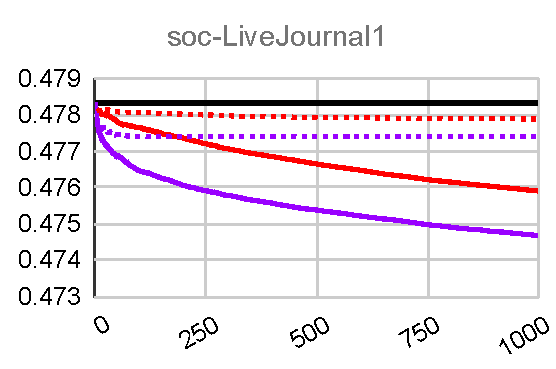
\includegraphics[width=0.23\linewidth]{out/im-soc-LiveJournal1.pdf}
  }
  \subfigure{
    \label{fig:im-coAuthorsDBLP}
    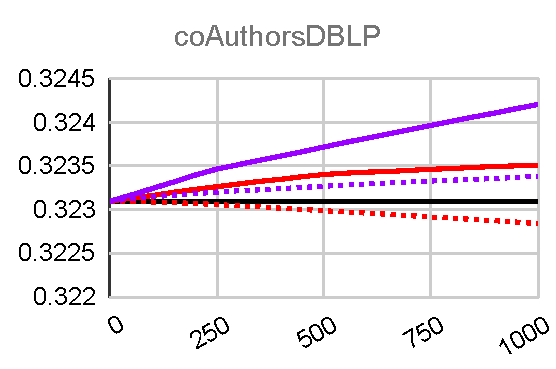
\includegraphics[width=0.23\linewidth]{out/im-coAuthorsDBLP.pdf}
  }
  \subfigure{
    \label{fig:im-coAuthorsCiteseer}
    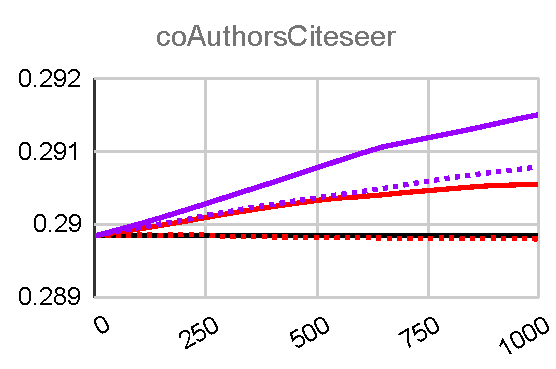
\includegraphics[width=0.23\linewidth]{out/im-coAuthorsCiteseer.pdf}
  }
  \subfigure{
    \label{fig:im-coPapersCiteseer}
    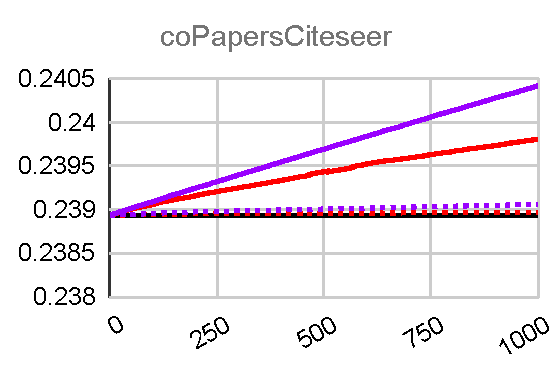
\includegraphics[width=0.23\linewidth]{out/im-coPapersCiteseer.pdf}
  }
  \subfigure{
    \label{fig:im-coPapersDBLP}
    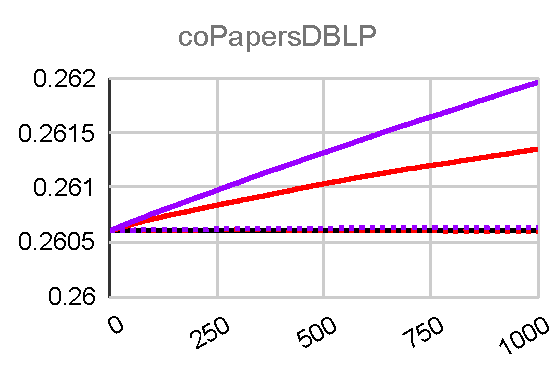
\includegraphics[width=0.23\linewidth]{out/im-coPapersDBLP.pdf}
  }
  \subfigure{
    \label{fig:im-italy_osm}
    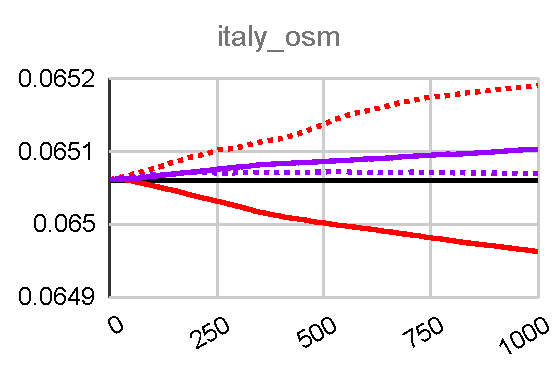
\includegraphics[width=0.23\linewidth]{out/im-italy_osm.pdf}
  }
  \subfigure{
    \label{fig:im-great-britain_osm}
    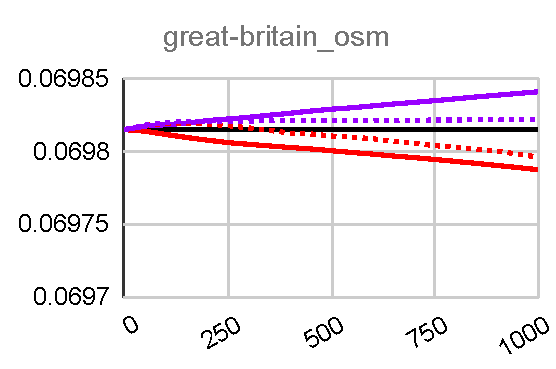
\includegraphics[width=0.23\linewidth]{out/im-great-britain_osm.pdf}
  }
  \subfigure{
    \label{fig:im-germany_osm}
    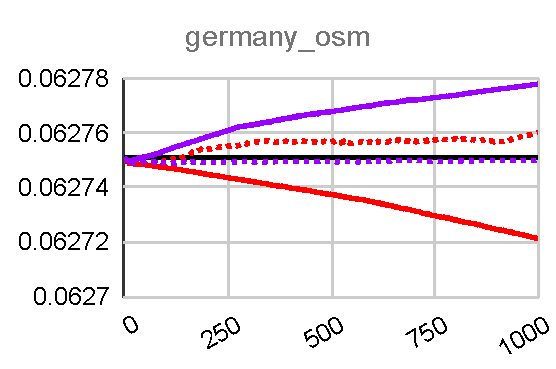
\includegraphics[width=0.23\linewidth]{out/im-germany_osm.pdf}
  }
  \subfigure{
    \label{fig:im-asia_osm}
    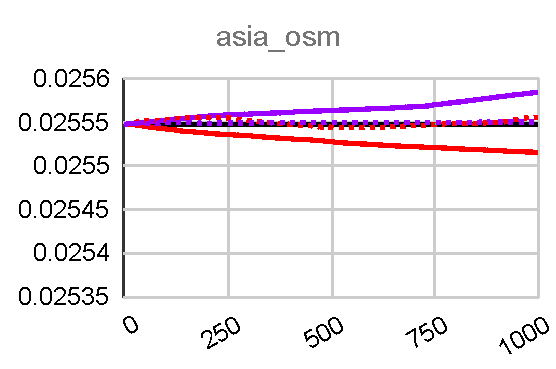
\includegraphics[width=0.23\linewidth]{out/im-asia_osm.pdf}
  }
  \subfigure{
    \label{fig:im-indochina-2004}
    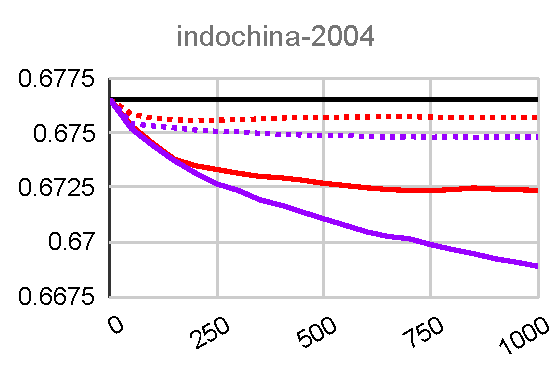
\includegraphics[width=0.23\linewidth]{out/im-indochina-2004.pdf}
  } \\[-2ex]
  \caption{Variation of Gini coefficient (Y-axis) with edges being added (X-axis) to the graphs incrementally with six different heuristics: \textit{edgeInsertCxrx}, \textit{edgeInsertCxSx}, \textit{edgeInsertCxSr}, \textit{edgeInsertCRrx}, \textit{edgeInsertCRSx}, and \textit{edgeInsertCRSr}.}
  \label{fig:im-all}
\end{figure*}
